%% ----------------------------------------------------------------------------
% BIWI SA/MA thesis template
%
% Created 09/29/2006 by Andreas Ess
% Extended 13/02/2009 by Jan Lesniak - jlesniak@vision.ee.ethz.ch
%% ----------------------------------------------------------------------------
\newpage
\chapter{Experiments and Results}
\label{sec:experimentsandresults}
Describe the evaluation you did in a way, such that an independent researcher can repeat it. Cover the following questions:
\begin{itemize}
    \item \textit{What is the experimental setup and methodology?} Describe the setting of the experiments and give all the parameters in detail which you have used. Give a detailed account of how the experiment was conducted.
    \item \textit{What are your results?} In this section, a \emph{clear description} of the results is given. If you produced lots of data, include only representative data here and put all results into the appendix.
\end{itemize}

\section{Training Models on MNIST, CIFAR and fastMRI}
In order to explore hyperparameters of the model architecture and debug the implementation it was decided to first train models on datasets considered trainable with less compute time. Two very well known datasets in computer vision that use low-resolution images are CIFAR10 and MNIST.~\autocite{cifar,mnist}
\begin{figure}[h]
    \centering
    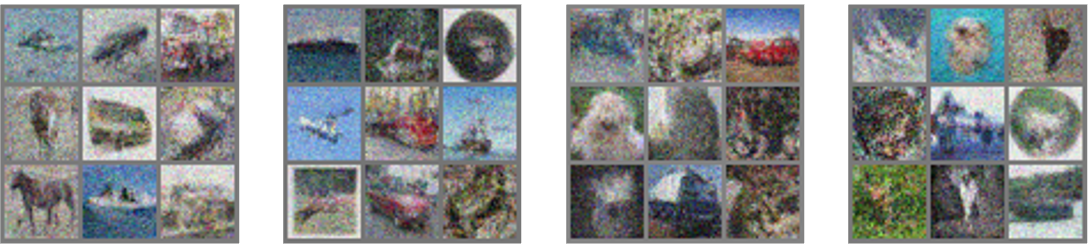
\includegraphics[width=.75\textwidth]{images/cifarsamples.png}
    \caption[Samples generated from CIFAR10]{Samples from the best performing model trained on CIFAR10 using a linear schedule: While the variance in the samples is large, suggesting that the model is able to capture the whole distribution, the samples are not completely denoised and therefore sample quality is seriously degenerated. As can be seen later, this was not observed when training on datasets where the image resolution was higher.}
    \label{fig:cifarsamples}
\end{figure}

\begin{figure}[h]
    \centering
    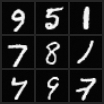
\includegraphics[width=.15\textwidth]{images/mnistsamples.png}
    \caption[Samples generated from MNIST]{Samples from the best performing model trained on MNIST}
    \label{fig:mnistsamples}
\end{figure}

Unconditional sampling was performed in order to verify the sample quality and whether the model was able to capture the main modes of the training data distribution. For a quantitative analysis of sample quality and mode coverage/log-likelihood of trained models Nichol et al. use FID score and Monte-Carlo log-likelihood estimates. FID requires the training of an additional classifier network, which only makes sense on standardized datasets with class labels such as ImageNet or CIFAR.~\autocite{imagenet, cifar} Pretrained classifiers are available for these datasets, which makes scores comparable among different generative models. The fastMRI dataset is not meant for classification tasks, therefore
\begin{figure}[h]
    \centering
    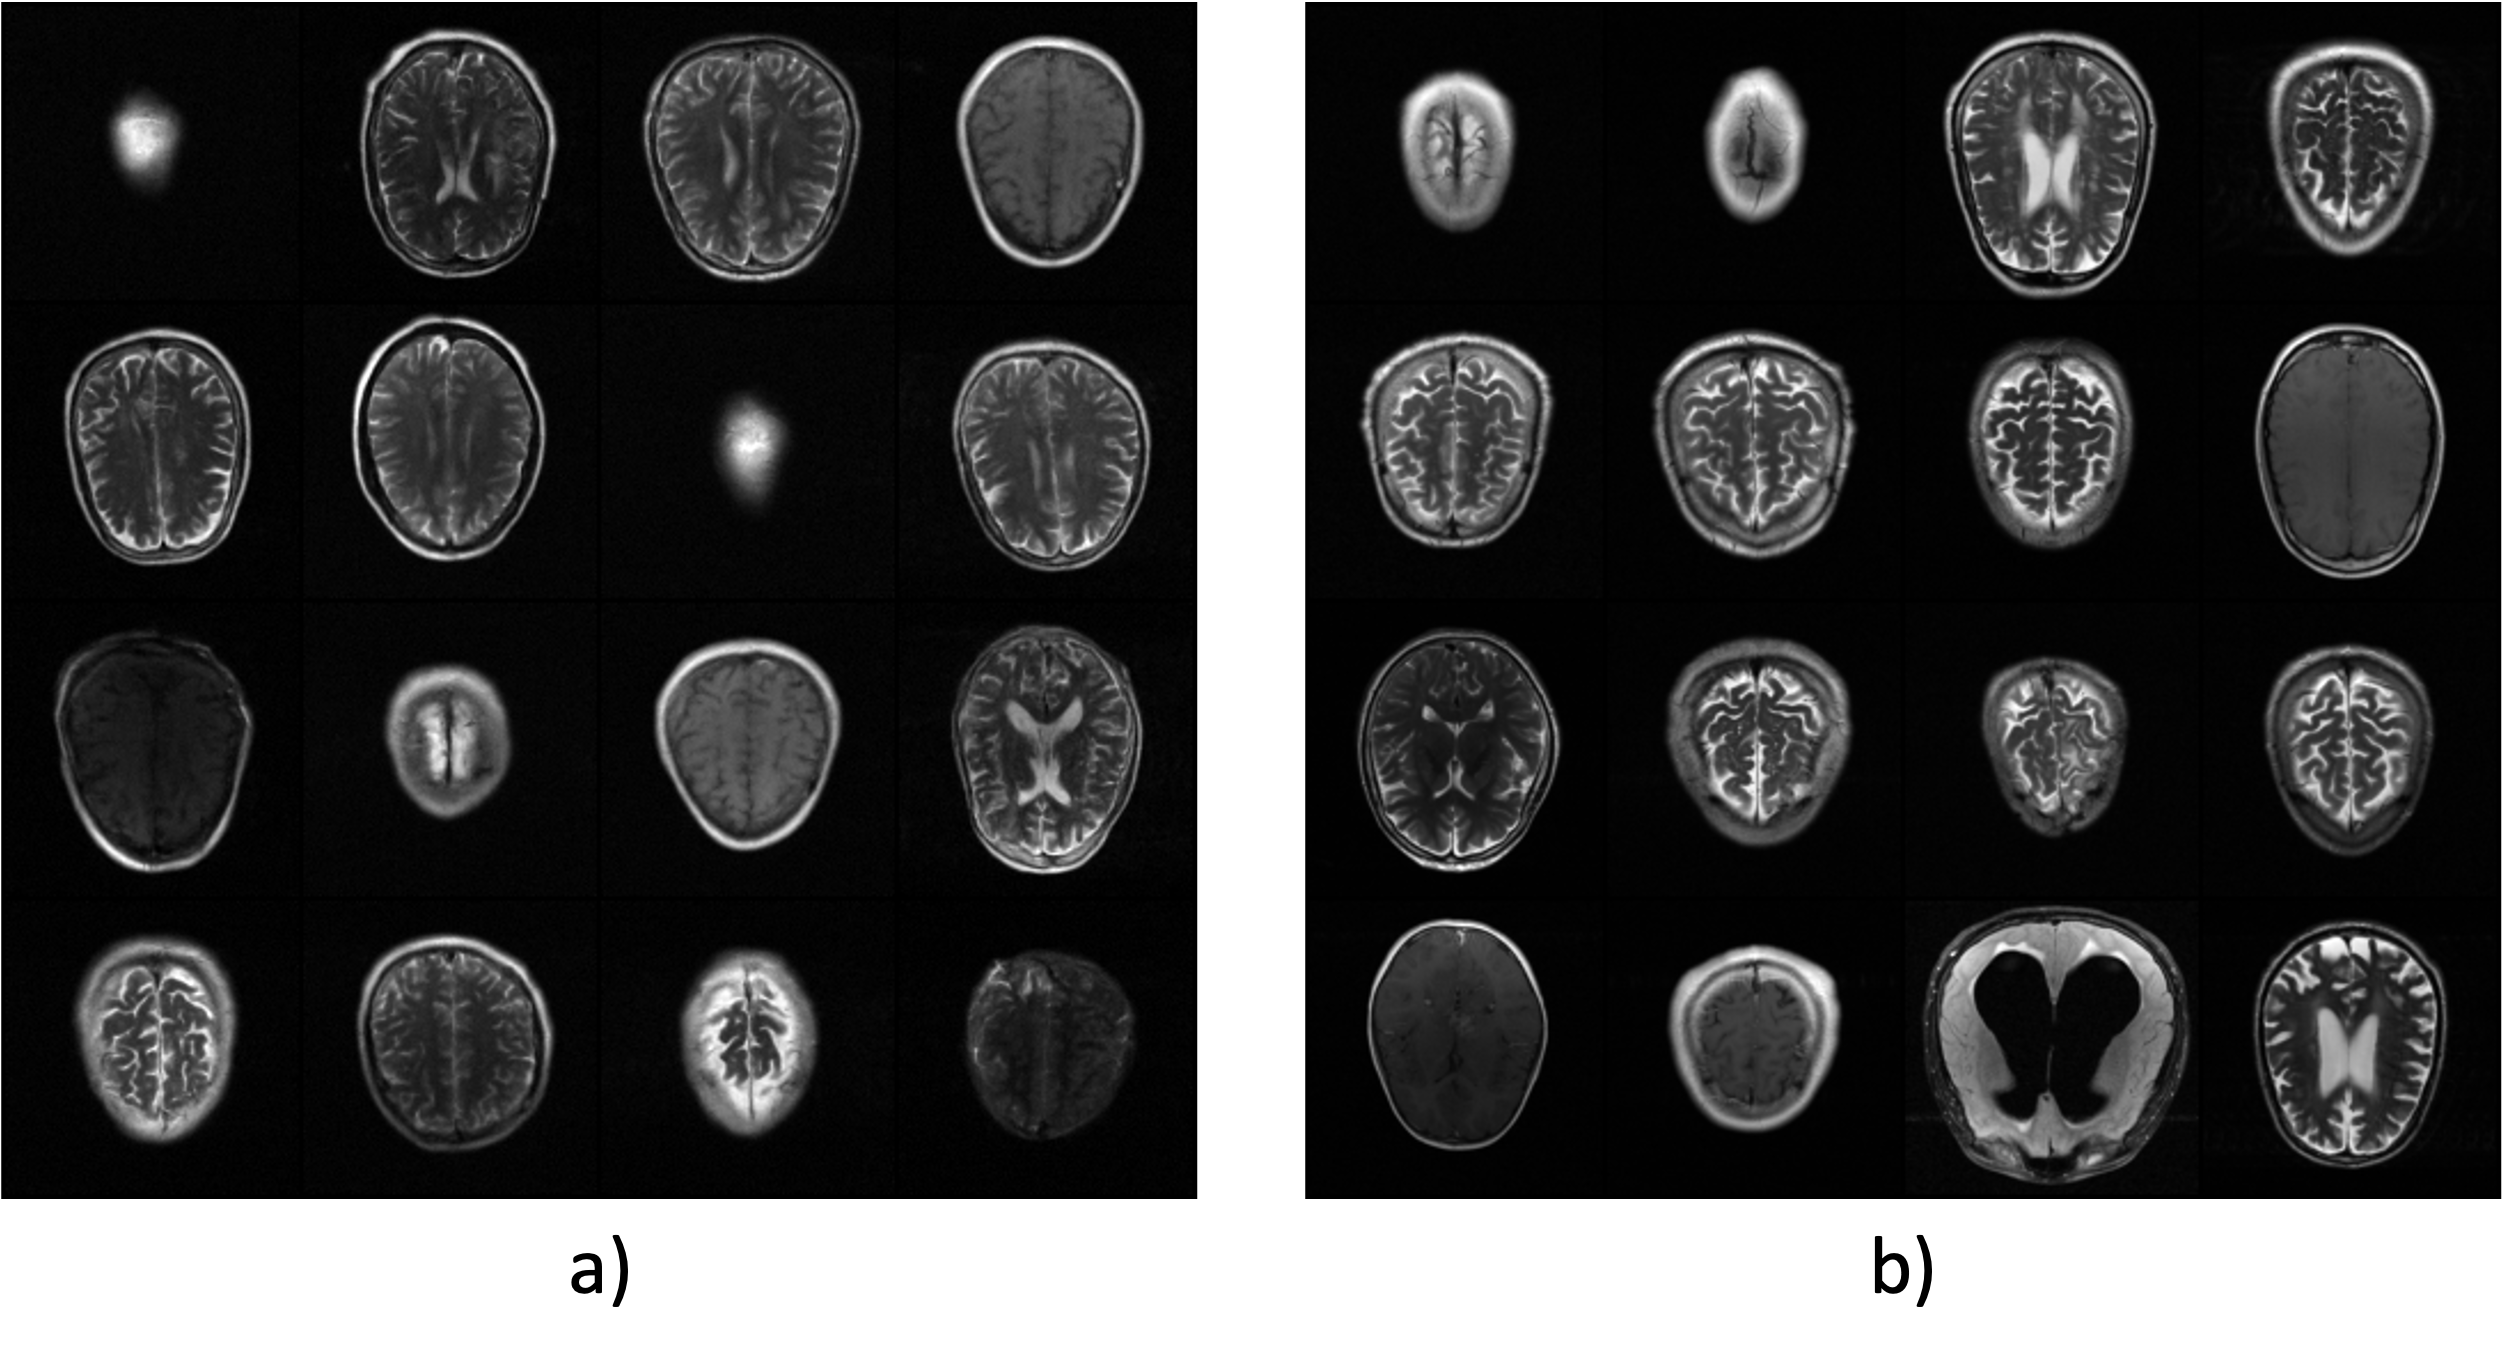
\includegraphics[width=.66\textwidth]{images/samples_unconditional.png}
    \caption[Samples from Data Set and Unconditional Sampling]{a) Unconditionally sampled examples, produced by the best-performing model; b) Examples from the training data set (fastMRI, RSS reconstruction); As can be seen, sample quality is comparable to the quality of the training samples and the variability among the samples is high, indicating a decent log-likelihood and mode coverage of the model.}
    \label{fig:uncondsampling}
\end{figure}

\section{Influence of Schedules and Image Size on the Forward Diffusion}
\label{sec:forward_diff_experiments}
Ho et al. had derived a closed form solution to the forward process of DDPMs and Nichol et al. investigated alternative options for the noise scheduling.~\autocite{ho2020denoising,nichol2021improved} They concluded that the important parameters to model are not the variances $\beta$ of the transitions, but the variances $1-\bar{\alpha}$ of the closed-form forward process, since they are the ones responsible for the destruction of information.

They decided to go with a squared cosine function, since this would be close to linear smooth out towards the critical beginning and end points of the process. In Fig.\ref{fig:alphadash} you can see how $1-\bar{\alpha}$ and $\beta$ behave for both approaches. It is immediately visible that the variances reach the maximum too early and flatten out for the linear schedule. This leads to the intuition that the last few steps are not very useful.

\begin{figure}[h]
    \centering
    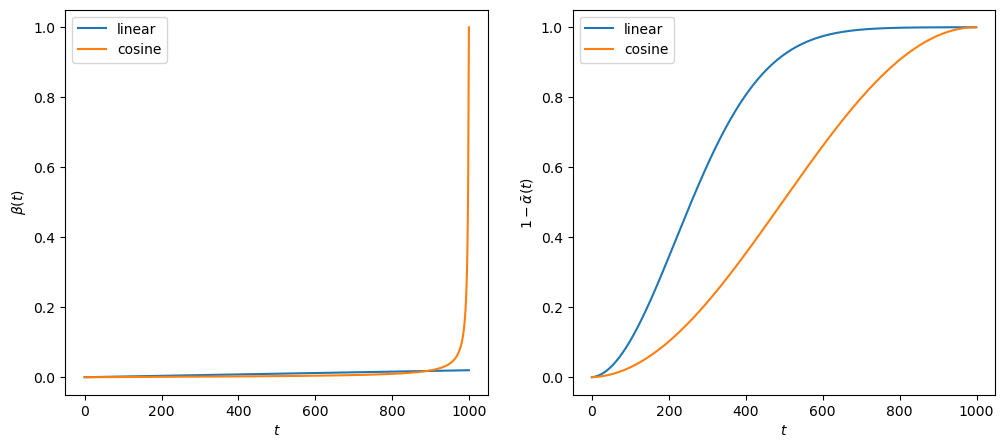
\includegraphics[width=.5\textwidth]{images/variance_schedule_alphadash.png}
    \caption{Variance Schedule Approaches: Modeling the $1-\bar{\alpha}$ as an approximate linear function (right cosine) and deriving $\beta$ (left cosine), or modeling $\beta$ as a linear function (left linear) and deriving $1-\bar{\alpha}$.}
    \label{fig:alphadash}
\end{figure}

The intution can experimentally confirmed by measuring how closely we get to isotropic noise when passing samples through the forward process. For this a batch of 50 times the same image was passed through the different steps of the process and the covariance matrix was calculated. As a metric for how close the covariance matrix was to the identity covariance matrix of pure i.i.d Gaussian noise, the identity matrix was subtracted and the mean of the absolute value of the matrix calculated. The results can be seen in Fig.~\ref{fig:noisecloseness} and confirm the intuition: When using linear scheduling we reach the closest point to pure noise already after around 600 steps for small images, and after around 700 for larger images. Cosine scheduling also performs worse on smaller images than on larger ones, but is still capable providing value for at least 850 timesteps.

\begin{figure}[h]
    \centering
    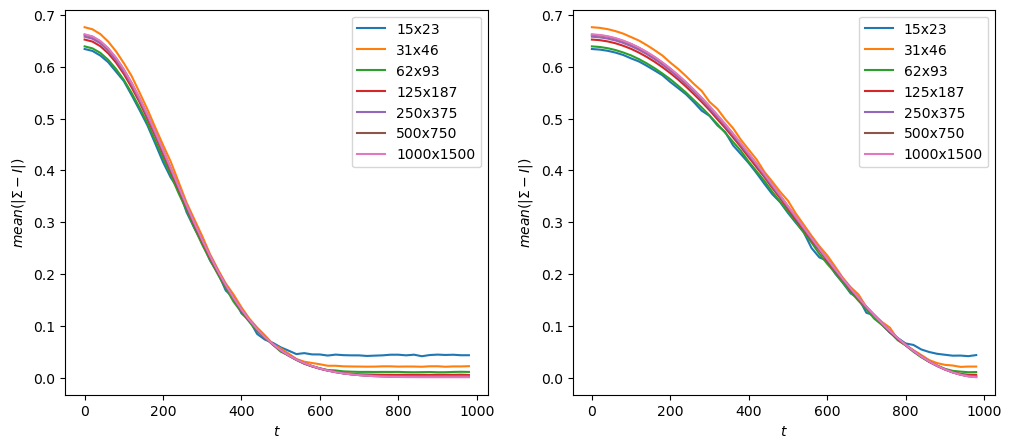
\includegraphics[width=.5\textwidth]{images/frobenius_norm.png}
    \caption{Closeness to noise for linear scheduling (left) and cosine scheduling (right).}
    \label{fig:noisecloseness}
\end{figure}

\section{Image Inpainting}
The work by Lugmayr et al.~\autocite{lugmayr2022repaint} was the main motivation to
\begin{figure}[h]
    \centering
    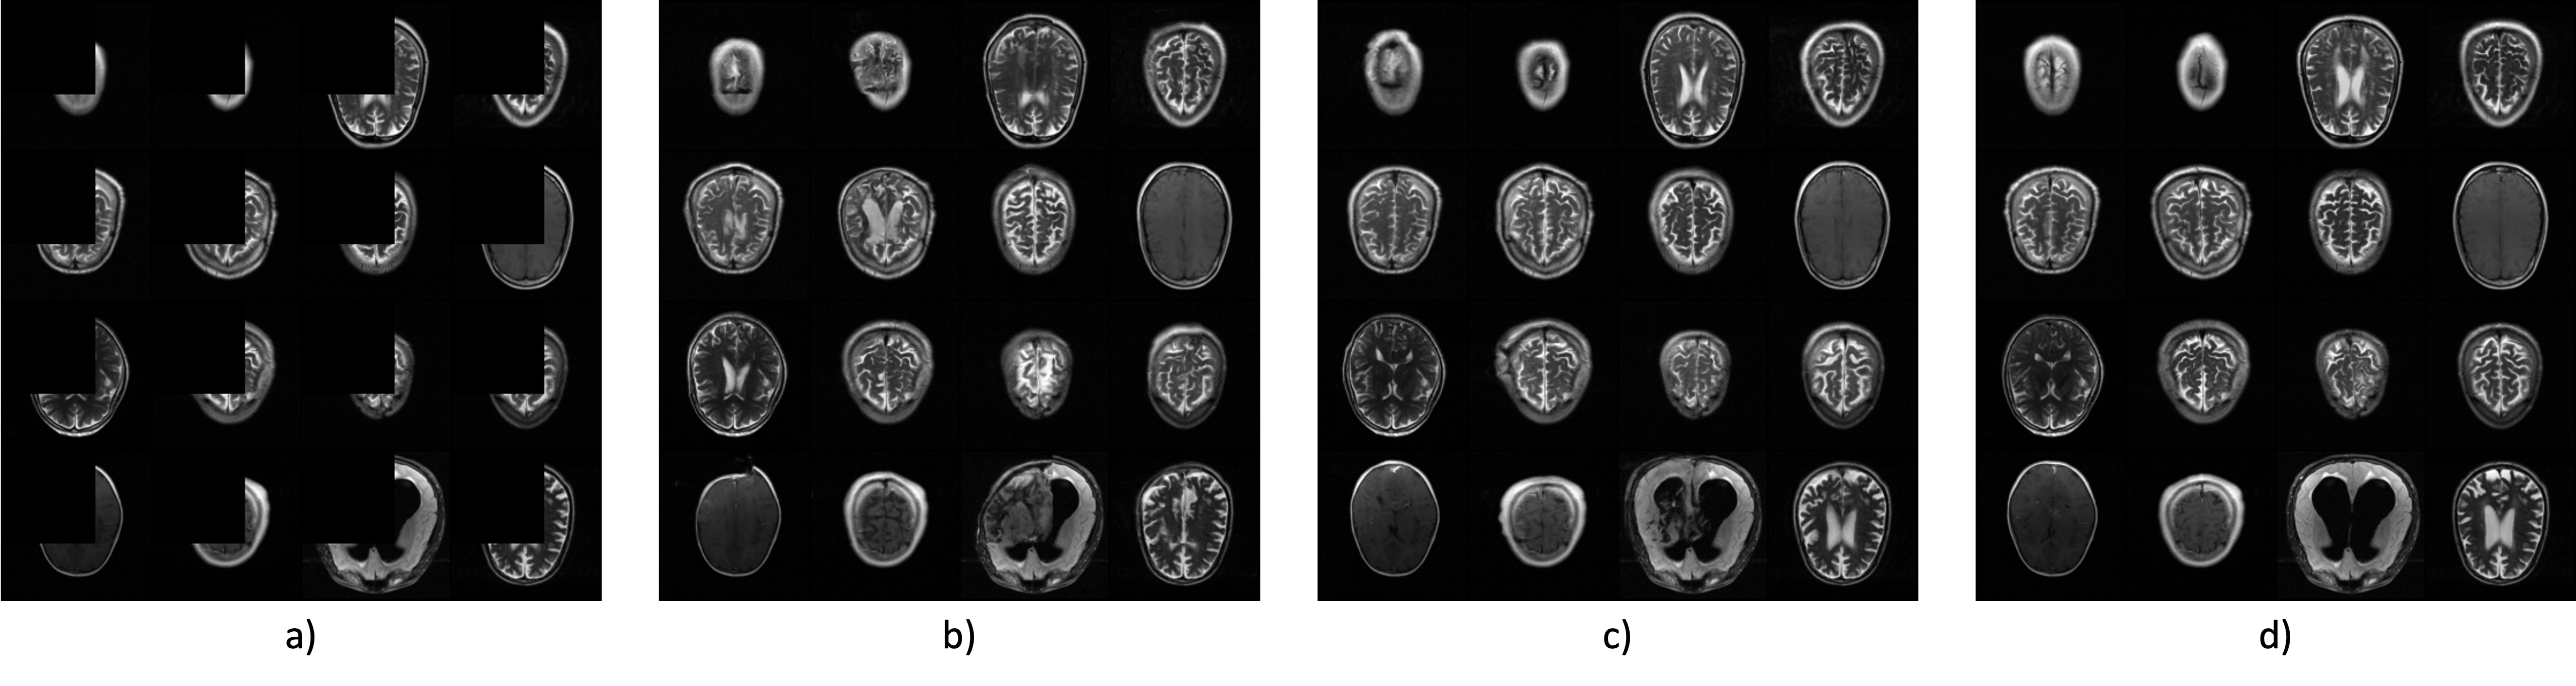
\includegraphics[width=.8\textwidth]{images/repaint.png}
    \caption[Inpainting and Resampling]{Inpainting and Resampling: a) Masked images used for the RePaint-style conditioning of the unconditional DDPM. b) Results from direct sampling. The reconstructed areas are often semantically wrong. c) Results from sampling with resampling. As observed by Lugmayr et al., the resampling strategy helps with semantically meaningful reconstruction. d) Ground truth images for comparison.}
\end{figure}

\section{Masked K-Space Substitution}
Lugmayr et al. use unconditional DDPMs to perform inpainting, which is a similar task to the reconstruction of undersampled MRI and are particularly successful by using resampling. This resampling process gives the network more time to create a globally semantically meaningful image.~\autocite{lugmayr2022repaint} Choi et al. replace low frequencies of the prediction with low frequencies of the latent representation of a target image to condition the diffusion process.~\autocite{choi2021ilvr} Since undersampled MRI still always contains global information, it was not expected, that resampling would have the same effect as with Lugmayr et al. Nevertheless it was expected to be an option for better sample fidelity through additional computation cost. The implementation follows below equation, where both, the latent prediction $x_t$ and the latent target $s_t$, are Fourier-transformed and predicted frequencies are replaced with known ones by the masking operation $\mathcal{M}$, wherever the information is available.
\begin{equation}
    x_{t-1} = x_t - \mathcal{F}^{-1}\left(\mathcal{M}\circ\mathcal{F}(x_t) + \mathcal{M}\circ\mathcal{F}(s_t)\right)
\end{equation}


\section{Variance in Predictions and Filtered Diffusion}
\label{sec:predvariance}
Aliasing arises from mismatches between predicted and introduced frequency information. Aliasing can be avoided by using low-pass filters, but the k-space mask is specifically sampled such that it also contains some information from higher frequencies. Naive low-pass filtering would make this information inaccessible and the sampling of those frequencies useless. Since the SNR (signal-to-noise-ratio) in natural images is much higher in the lower frequencies than in the lower ones, it was hypothesized that it might be possible to add frequency information gradually during the denoising process in order to avoid aliasing, lower frequencies first and higher ones only towards the end.

In order to empirically study this hypothesis, a single sample was denoised and its latent representations at every 10th timestep were saved. These latent representations were copied into batches of 100 equal latent representations and the denoising process was continued for all these batches. Fig.~\ref{fig:predvariance} shows 4 of these samples for a subset of starting points. As can be seen, when starting from $t\geq700$, the samples still have a lot of variability and share very few features. When starting later in the process, the samples look already very similar and only differ in some details. Since high frequencies are responsible for carrying information on details, this supports the hypothesis, but it becomes more evident, when looking at the variances of the spectral representations as seen in Fig.~\ref{fig:spectralvariance}. The variances were estimated over the frequency representations of all the final predictions in a batch (100 samples, denoised from $t$) and high variance means that this frequency was not yet determined at that specific $t$. As can be clearly seen in the figure, the variance is concentrated in the low frequencies when starting at larget $t$, and the variance in the low frequencies increases as the starting $t$ decreases. This again supports the hypothesis that high frequencies matter much more towards the end and that it might be possible to only introduce them later in the process.
\begin{figure}[h]
    \centering
    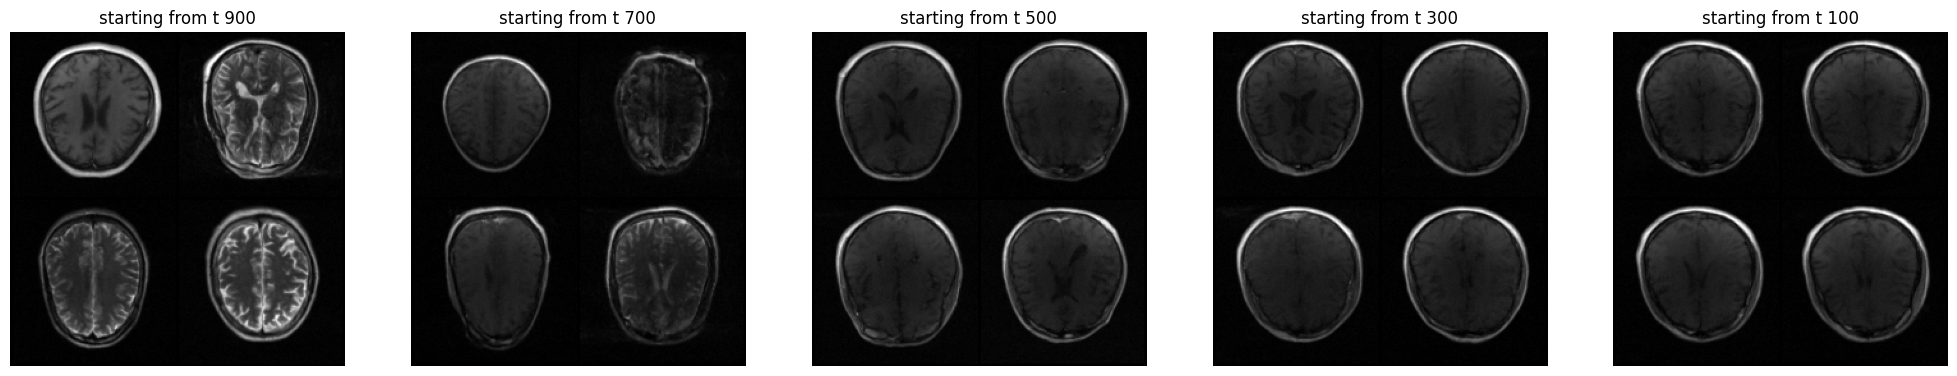
\includegraphics[width=.75\textwidth]{images/fixedlatents_variance.png}
    \caption[Variance in Predictions from Fixed Latents]{Variance in Predictions from Fixed Latents: The general shape of the final samples is already determined at $t=500$ and from there, the variability in the outputs is mostly about details of the structure.}
    \label{fig:predvariance}
\end{figure}

\begin{figure}[h]
    \centering
    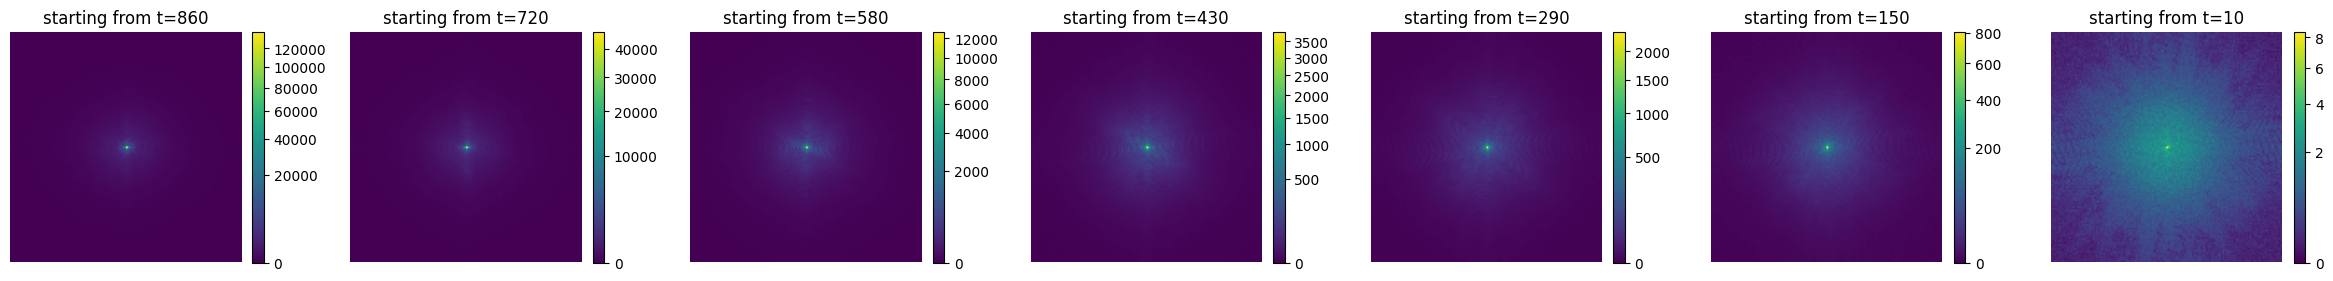
\includegraphics[width=\textwidth]{images/fixedlatents_varSpectra.png}
    \caption[Spectral Variance from Fixed Latents]{Variance in the Spectra when starting from Fixed Latents: When generating samples from fixed latent representation early in the denoising process, the variance of the spatial frequencies is highly concentrated in the center (e.g. $t=860$), overpowering the variance in the low frequencies by several orders of magnitude. The differences are smaller when starting late in the process (e.g. $t=10$), suggesting that fine details are only reconstructed at the very end. This hypothesis is also supported by the fact that natural images have lower SNR in the higher frequencies, which means that Gaussian perturbation affects them more and they can't carry much information until most of the noise is removed.}
    \label{fig:spectralvariance}
\end{figure}
\section{Frequency Replacement vs. Loss Function Guidance}
Results from section~\ref{sec:predvariance} suggested that lower frequencies only matter towards the end of the denoising process and guided diffusion with a loss function provides an additional to look at this by inspecting the gradients. Since these gradients are very noisy, they were averaged over a batch of 1200 equal samples. The results have been can be seen in Fig~\ref{fig:lossgradients} of the appendix.

\begin{figure}[h]
    \centering
    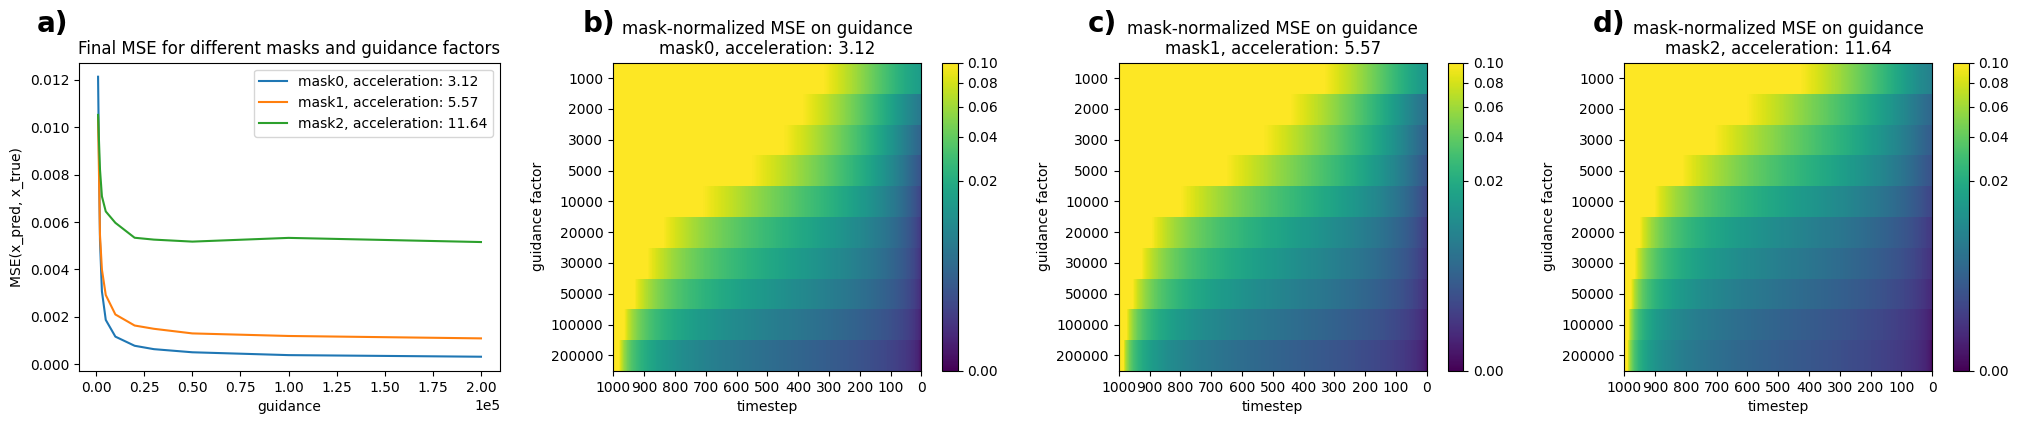
\includegraphics[width=\textwidth]{images/direct_sampling.png}
    \caption[Direct Sampling with Loss Guidance]{Results from Direct Sampling with Loss Guidance.}
\end{figure}